\chapter{La théorie de Ramsey}\label{c.ramsey}



%%%%%%%%%%%%%%%%%%%%%%%%%%%%%%%%%%%%%%%%%%%%%%%%%%%%%%%%%%%

La théorie de Ramsey est une branche de la combinatoire qui pose des questions de la forme suivante : quelle doit être la taille d'un ensemble pour que, si on le divise en sous-ensembles, au moins un sous-ensemble ait une certaine propriété ?
Les résultats de la théorie de Ramsey sont difficiles à démontrer et de nombreux problèmes restent ouverts. Dans ce chapitre, nous présentons des cas simples de quatre problèmes pour donner un aperçu de ce sujet fascinant : les triplets de Schur (sect.~\ref{s.schur}), des triplets d'entiers tels que $a+b=c$; les triplets de Pythagore (sect.~\ref{s.pyth}), des triplets d'entiers tels que $a^2+b^2=c^2$; le problème de van der Waarden (sect.~\ref{s.van}) qui concerne les suites de nombres; le théorème de Ramsey (sect.~\ref{s.ramsey}) sur le coloriage des graphes. La section~\ref{s.bounds} montre comment la méthode probabiliste en combinatoire permet de trouver une borne inférieure pour les nombres de Ramsey.

Le problème des triplets pythagoriciens a récemment été résolu à l'aide d'ordinateurs, en utilisant une méthode relativement nouvelle appelée résolution SAT. Pour les lecteurs familiers avec la logique propositionnelle, la section \ref{s.sat} donne un aperçu de la méthode utilisée.

La section~\ref{s.plimpton} décrit les triplets pythagoriciens tels qu'ils étaient connus des Babyloniens il y a quatre mille ans.

Terminologie : \emph{monochromatique} signifie de la même couleur.

%%%%%%%%%%%%%%%%%%%%%%%%%%%%%%%%%%%%%%%%%%%%%%%%%%%%%%%%%%%


\section{Les triplets de Schur}\label{s.schur}


\begin{definition}
Étant donné une décomposition quelconque de l'ensemble des entiers strictement positifs  
$S(n)=\{1,\ldots,n\}$ 
en deux sous-ensembles disjoints $S_1$ et $S_2$, existe-t-il $\{a,b,c\}\subseteq  S_1$ ou $\{a,b,c\}\subseteq S_2$ (ou les deux) tel que $a\!<\!b\!<\!c$ et $a+b=c$ ? Si oui, l'ensemble $\{a,b,c\}$ est appelé un \emph{triplet de Schur}.
\end{definition}

\begin{example} Pour $n=8$, dans la décomposition 
\begin{align}
S_1 = \{1,2,3,4\},\; S_2 = \{5,6,7,8\}\,,
\label{eq.schur0}
\end{align}
l'ensemble $S_1$ comprend le triplet de Schur $\{1,2,3\}$.
Cependant, la décomposition 
\begin{align}
S'_1 = \{1,2,4,8\},\; S'_2 = \{3,5,6,7\}\,,
\label{eq:schur1}
\end{align}
ne contient pas de triplet de Schur, comme on peut le vérifier en énumérant tous les triplets de chaque sous-ensemble.
\end{example}

\begin{theorem}
Dans toutes les décompositions de $S(9)=\{1,\ldots,9\}$ en deux sous-ensembles disjoints, au moins un sous-ensemble contient un triplet de Schur.
\end{theorem}
Bien sûr, nous pourrions vérifier les $2^9=512$ décompositions de $S(9)$ en deux sous-ensembles disjoints, mais essayons de trouver une démonstration plus succincte.
\begin{proof}
Nous essayons de construire une décomposition qui ne contient pas de triplet de Schur et montrons que les contraintes du problème rendent cela impossible. Commençons par placer $1$ et $3$ dans le sous-ensemble $S_1$. $2$ doit être placé dans $S_2$ car $1+2=3$ et nous essayons de construire une décomposition qui ne contient pas de triplet de Schur. De même, $4$ doit être placé dans $S_2$ car $1+3=4$. En continuant, $6$ est placé dans $S_1$ car $2+4=6$ et $7$ est placé dans $S_2$ car $1+6=7$. Cependant, $3+6=9$ et $2+7=9$, donc $9$ doit apparaître à la fois dans $S_1$ et $S_2$, une contradiction. La suite des déductions est présentée dans le tableau suivant :
\[
\begin{array}{l@{\hspace{2em}}l}
S_1&S_2\\ \hline
1,3 & \\
1,3 & 2\\
1,3 & 2,4\\
1,3,6 & 2,4\\
1,3,6 & 2,4,7\\
1,3,6,9 & 2,4,7\\
1,3,6,9 & 2,4,7,9
\end{array}
\]
En revenant en arrière, nous cherchons une décomposition où $1$ et 3 sont dans des sous-ensembles différents. Si nous plaçons $5$ dans $S_2$, une suite d'inférences conduit à nouveau à une contradiction car $9$ doit apparaître dans les deux sous-ensembles. Le lecteur doit justifier chacune des inférences présentées dans le tableau suivant :
\[
\begin{array}{l@{\hspace{2em}}l}
S_1&S_2\\
1&3\\
1 & 3,5\\
1,2&3,5\\
1,2,8&3,5\\
1,2,8&3,5,7\\
1,2,8&3,5,7,9\\
1,2,8&3,5,6,7,9\\
1,2,8,9&3,5,6,7,9
\end{array}
\]


En revenant en arrière, nous essayons de placer $5$ dans $S_1$, mais cela conduit également à une contradiction, comme le montre le tableau suivant :
\[
\begin{array}{l@{\hspace{2em}}l}
S_1&S_2\\\hline
1&3\\
1,5& 3\\
1,5&3,4\\
1,5&3,4,6\\
1,2,5&3,4,6\\
1,2,5&3,4,6,7\\
1,2,5,7&3,4,6,7
\end{array}
\]

Par conséquent, il n'existe aucune décomposition qui n'inclut pas un triplet de Schur.
\end{proof}
 Issaï Schur a démontré le théorème suivant :
\begin{theorem}[Schur]
Pour tout $k\geq 2$, il existe un plus petit $n$ tel que dans toute décomposition disjointe de $S(n)$ en $k$ sous-ensembles, au moins un des sous-ensembles doit contenir un triplet de Schur.
\end{theorem}


\section{Les triplets pythagoriciens  }\label{s.pyth}

\begin{definition}
Étant donné une décomposition quelconque de l'ensemble des  entiers strictement positifs $S(n)=\{1,\ldots,n\}$ 
en deux sous-ensembles disjoints $S_1$ et $S_2$, existe-t-il $\{a,b,c\}\subseteq S_1$ ou $\{a,b,c\}\subseteq S_2$ (ou les deux) tel que $a\!<\!b\!<\!c$ et $a^2+b^2=c^2$ ? Si oui, $\{a,b,c\}$ est appelé un \emph{triplet pythagoricien}.
\end{definition}

\begin{example}
Pour $n=10$, dans la décomposition en nombres pairs et impairs 
\[
S_1 = \{1,3,5,7,9\},\; S_2=\{2,4,6,8,10\}\,,
\]
il n'y a pas de triplets pythagoriciens dans $S_1$ mais $\{6,8,10\}$ dans $S_2$ est un triplet pythagoricien puisque $6^2+8^2=10^2$.
\end{example}

Marijn J.\,H. Heule et Oliver Kullmann ont démontré les théorèmes suivants. Leur méthode de démonstration est expliquée dans la section~\ref{s.sat}.

\begin{theorem}
Pour tout $n\leq 7\,824$, il existe une  décomposition de $S(n)$ en deux sous-ensembles disjoints telle que les deux sous-ensembles ne contiennent pas de triplet pythagoricien.
\end{theorem}

\begin{theorem}
Pour tout $n\geq 7\,825$, dans toute décomposition de $S(n)$ en deux sous-ensembles disjoints, au moins un sous-ensemble contient un triplet pythagoricien.
\end{theorem}
Il est impossible de vérifier toutes les $2^{7\,825}$ décompositions de $S(7\,825)$. Si nous pouvions vérifier une décomposition toutes les microsecondes, $2^{7\,825}\; \textrm{microsecondes}\approx 10^{600}\; \textrm{années}$, alors que l'âge estimé de l'univers n'est que d'environ $10^{10}$ années.



%%%%%%%%%%%%%%%%%%%%%%%%%%%%%%%%%%%%%%%%%%%%%%%%%%%%%%%%%%%

\section{Le problème de van der Waerden}\label{s.van}

Considérons les suites de huit points coloriés de la figure~\ref{f.vdw1}. Dans la suite du haut, il y a des points rouges aux positions $(1,2,3)$ et des points bleus aux positions $(4,5,6)$. Dans chaque cas, les positions forment une progression arithmétique. De même, dans la suite du milieu, les points rouges aux positions $(1,3,5)$ forment une progression arithmétique. Cependant, dans la suite du bas, il n'existe pas d'ensemble de trois points monochromatiques dont les positions forment une progression arithmétique. 
Les triplets de points rouges se trouvent aux positions $(1,2,5)$, $(1,2,6)$, $(2,5,6)$, dont aucune ne forme de progression arithmétique, et de même pour les points bleus.

\begin{figure}[htb]
\centering
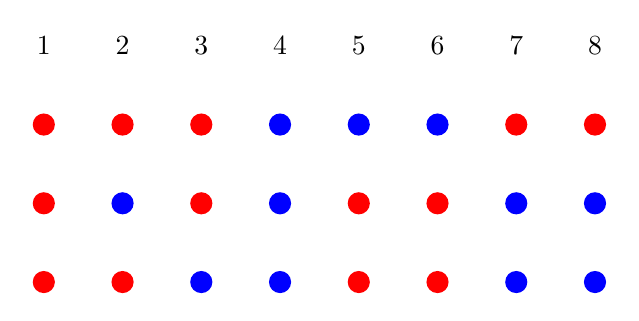
\begin{tikzpicture}
\foreach \x in {1,2,3,4,5,6,7,8} {
  \node at (\x,3) {$\x$};
}
\foreach \x/\col in {1/red,2/red,3/red,4/blue,5/blue,6/blue,7/red,8/red} {
  \fill[\col] (\x,2) circle(4pt);
}
\foreach \x/\col in {1/red,2/blue,3/red,4/blue,5/red,6/red,7/blue,8/blue} {
  \fill[\col] (\x,1) circle(4pt);
}
\foreach \x/\col in {1/red,2/red,3/blue,4/blue,5/red,6/red,7/blue,8/blue} {
  \fill[\col] (\x,0) circle(4pt);
}
\end{tikzpicture}
%\includegraphics[width=0.8\textwidth]{Fig8_1}
\caption{Le problème de van der Waerden pour huit points coloriés.}\label{f.vdw1}
\end{figure}

Avec neuf points, tout coloriage doit contenir une suite de trois points monochromatiques qui forment une progression arithmétique. Par exemple, ajoutons un point rouge ou un point bleu à la fin de la suite du bas de la figure~\ref{f.vdw1} pour obtenir les suites de la figure~\ref{f.vdw2}. Dans la suite du haut, il y a des points rouges aux positions $(1,5,9)$, une progression arithmétique, et dans la suite du bas, il y a des points bleus aux positions $(7,8,9)$, également une progression arithmétique.

\begin{figure}[htb]
\centering
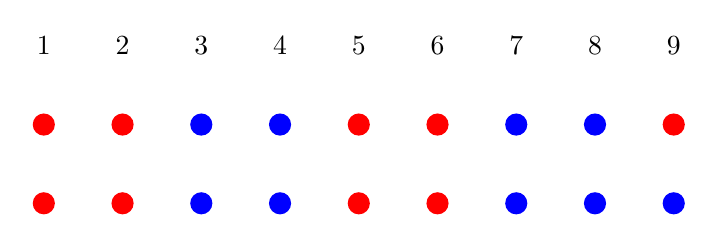
\begin{tikzpicture}
\foreach \x in {1,2,3,4,5,6,7,8,9} {
  \node at (\x,2) {$\x$};
}
\foreach \x/\col in {1/red,2/red,3/blue,4/blue,5/red,6/red,7/blue,8/blue,9/red} {
  \fill[\col] (\x,1) circle(4pt);
}
\foreach \x/\col in {1/red,2/red,3/blue,4/blue,5/red,6/red,7/blue,8/blue,9/blue} {
  \fill[\col] (\x,0) circle(4pt);
}
\end{tikzpicture}
%\includegraphics[width=\textwidth]{Fig8_2}
\caption{Le problème de van der Waerden pour neuf points coloriés.}\label{f.vdw2}
\end{figure}


Bartel L. van der Waerden a posé le problème suivant : pour tout entier strictement positif $k$, quel est le plus petit nombre $n$ tel que toute suite de $n$ points coloriés doit contenir une suite de $k$ points monochromatiques qui forment une progression arithmétique ? Pour $k=3$, on a $n=9$, comme démontré ci-dessus pour une décomposition. Le résultat suivant est plus difficile à démontrer : pour $k=4$, on a $n=35$.


%%%%%%%%%%%%%%%%%%%%%%%%%%%%%%%%%%%%%%%%%%%%%%%%%%%%%%%%%%%


\section{Le théorème de Ramsey}\label{s.ramsey}

Colorions les arêtes de $K_5$, le graphe complet à 5 sommets, avec deux couleurs comme indiqué sur la figure~\ref{f.ramsey5}. Il n'y a pas de sous-graphes monochromatiques $K_3$ (triangles) dans le graphe. La figure~\ref{f.ramsey6} montre un coloriage de $K_6$ et il est facile de voir qu'il existe des triangles monochromatiques $\triangle ACE$ et $\triangle BDF$. Dans cette section, nous démontrons un cas simple d'un théorème de Frank P. Ramsey sur l'existence de sous-ensembles ayant une certaine propriété.


\vspace{0.4cm}

\begin{minipage}{0.4\textwidth}
\centering     
\begin{tikzpicture}
\node (pentagon) [minimum size=4.5cm,regular polygon,regular polygon sides=5] at (0,0) {};
\draw[red]  (pentagon.corner 1) node[black,above] {$A$} -- (pentagon.corner 2);
\draw[red]  (pentagon.corner 2) node[black,left] {$B$} -- (pentagon.corner 3);
\draw[red]  (pentagon.corner 3) node[black,left] {$C$} -- (pentagon.corner 4);
\draw[red]  (pentagon.corner 4) node[black,right] {$D$} -- (pentagon.corner 5);
\draw[red]  (pentagon.corner 5) node[black,right] {$E$} -- (pentagon.corner 1);
\draw[dashed,blue] (pentagon.corner 1) -- (pentagon.corner 3);
\draw[dashed,blue] (pentagon.corner 1) -- (pentagon.corner 4);
\draw[dashed,blue] (pentagon.corner 2) -- (pentagon.corner 4);
\draw[dashed,blue] (pentagon.corner 2) -- (pentagon.corner 5);
\draw[dashed,blue] (pentagon.corner 3) -- (pentagon.corner 5);
\end{tikzpicture}
%\includegraphics[width=\textwidth]{Fig8_3a}
         \captionof{figure}{Un coloriage de $K_5$ avec deux couleurs.}\label{f.ramsey5}
         
     \end{minipage}
     \hspace{3em}
     \begin{minipage}{0.4\textwidth}
\centering  
\begin{tikzpicture}
\node (hexagon) [minimum size=4.5cm,regular polygon,regular polygon sides=6] at (0,0) {};
\draw[red]  (hexagon.corner 1) node[black,above] {$A$} -- (hexagon.corner 2);
\draw[red]  (hexagon.corner 2) node[black,above] {$B$} -- (hexagon.corner 3);
\draw[red]  (hexagon.corner 3) node[black,left] {$C$} -- (hexagon.corner 4);
\draw[red]  (hexagon.corner 4) node[black,left] {$D$} -- (hexagon.corner 5);
\draw[red]  (hexagon.corner 5) node[black,right] {$E$} -- (hexagon.corner 6);
\draw[red]  (hexagon.corner 6) node[black,right] {$F$} -- (hexagon.corner 1);
\draw[dashed,blue] (hexagon.corner 1) -- (hexagon.corner 3);
\draw[dashed,blue] (hexagon.corner 1) -- (hexagon.corner 4);
\draw[dashed,blue] (hexagon.corner 1) -- (hexagon.corner 5);
\draw[dashed,blue] (hexagon.corner 2) -- (hexagon.corner 4);
\draw[dashed,blue] (hexagon.corner 2) -- (hexagon.corner 5);
\draw[dashed,blue] (hexagon.corner 2) -- (hexagon.corner 6);
\draw[dashed,blue] (hexagon.corner 3) -- (hexagon.corner 5);
\draw[dashed,blue] (hexagon.corner 3) -- (hexagon.corner 6);
\draw[dashed,blue] (hexagon.corner 4) -- (hexagon.corner 6);
\end{tikzpicture}
%\includegraphics[width=\textwidth]{Fig8_3b}
         \captionof{figure}{Un coloriage de $K_6$ avec deux couleurs.}\label{f.ramsey6}
     \end{minipage}

\vspace{0.4cm}





\begin{definition}
 Le nombre de Ramsey pour $k$,  $R(k)$, est le plus petit nombre $n$ tel que dans tout coloriage avec deux couleurs de $K_{n}$, le graphe complet à $n$ sommets,  il existe un sous-graphe complet monochromatique $K_k$.
\end{definition}


\begin{theorem}[Ramsey]
$\quad R(3)=6$.\label{thm.ramsey}
\end{theorem}

\begin{proof} 
La figure~\ref{f.ramsey5} montre que $R(3)>5$. Pour montrer que $R(3)\leq 6$, considérons un sommet quelconque $s$ dans $K_6$. Le sommet $s$ est relié à cinq autres sommets, et lorsque les arêtes sont coloriées avec deux couleurs, il doit y avoir au moins trois arêtes monochromatiques qui arrivent en $s$. 

Sur la figure~\ref{f.ramsey4a}, les arêtes $\overline{AB}$, $\overline{AC}$ et $\overline{AE}$ sont coloriées en rouge. Puisque le graphe est complet, tous les sommets sont reliés, donc si l'une des arêtes $\overline{BC}$, $\overline{BE}$ ou $\overline{CE}$ est coloriée en rouge, disons $\overline{BE}$, un triangle rouge $\triangle ABE$ se forme. Sinon, les trois arêtes sont coloriées en bleu et forment un triangle bleu (fig.~\ref{f.ramsey4b}).
\end{proof}

Le théorème se généralise à un nombre quelconque de couleurs, ainsi qu'à des coloriages où les tailles des sous-graphes ne sont pas les mêmes. $R(r,b,v)$ est le plus petit graphe complet tel que dans tout coloriage à trois couleurs, il doit y avoir des sous-graphes complets avec $r$ arêtes rouges, $b$ arêtes bleues et $v$ arêtes vertes.

\vspace{0.4cm}

\begin{minipage}{0.4\textwidth}
\centering     
\begin{tikzpicture}
\node (hexagon) [minimum size=4.5cm,regular polygon,regular polygon sides=6] at (0,0) {};
\draw[red]  (hexagon.corner 1) node[black,above] {$A$} -- (hexagon.corner 2) node[black,above] {$B$};
\draw[blue,dashed]  (hexagon.corner 1) -- (hexagon.corner 6) node[black,right] {$F$};
\draw[red] (hexagon.corner 1) -- (hexagon.corner 3) node[black,below] {$C$};
\draw[blue,dashed] (hexagon.corner 1) -- (hexagon.corner 4) node[black,right] {$D$};
\draw[red] (hexagon.corner 1) -- (hexagon.corner 5) node[black,right] {$E$};
\end{tikzpicture}
%\includegraphics[width=\textwidth]{Fig8_4a}
         \captionof{figure}{Un sommet de $K_6$.}\label{f.ramsey4a}
         
     \end{minipage}
     \hspace{3em}
     \begin{minipage}{0.4\textwidth}
\centering        
\begin{tikzpicture}
\node (hexagon) [minimum size=4.5cm,regular polygon,regular polygon sides=6] at (0,0) {};
\draw[very thick,red]  (hexagon.corner 1) node[black,above] {$A$} -- (hexagon.corner 2) node[black,above] {$B$};
\draw[blue,dashed]  (hexagon.corner 1) -- (hexagon.corner 6) node[black,right] {$F$};
\draw[red] (hexagon.corner 1) -- (hexagon.corner 3) node[black,below] {$C$};
\draw[blue,dashed] (hexagon.corner 1) -- (hexagon.corner 4) node[black,right] {$D$};
\draw[very thick,red] (hexagon.corner 1) -- (hexagon.corner 5) node[black,right] {$E$};
\draw[very thick,red] (hexagon.corner 2) -- (hexagon.corner 5);
\draw[very thick,blue,dashed] (hexagon.corner 2) -- (hexagon.corner 3);
\draw[very thick,blue,dashed] ($(hexagon.corner 2)+(-2pt,0)$) -- ($(hexagon.corner 5)+(-2pt,0)$);
\draw[very thick,blue,dashed] (hexagon.corner 5) -- (hexagon.corner 3);
\end{tikzpicture}
%\includegraphics[width=\textwidth]{Fig8_4b}
         \captionof{figure}{Triangles mono\-chromatiques dans $K_6$.}\label{f.ramsey4b}
     \end{minipage}



%%%%%%%%%%%%%%%%%%%%%%%%%%%%%%%%%%%%%%%%%%%%%%%%%%%%%%%%%%%

\section{La méthode probabiliste}\label{s.bounds}

Les seuls nombres de Ramsey non triviaux connus sont $R(3)=6$ et $R(4)=18$. En 1947, Paul Erd\H{o}s a introduit la méthode probabiliste et l'a utilisée pour établir des limites inférieures et supérieures pour $R(k)$. Des recherches ultérieures ont permis d'améliorer ces deux bornes, mais il s'agit toujours d'un domaine de recherche important car les bornes ne sont pas étroites. Par exemple, on a démontré que $43\leq R(5) \leq 48$ et $798\leq R(10)\leq 23\,556$. Dans cette section, on utilise les probabilités élémentaires pour obtenir une borne inférieure sur $R(k)$.

Pour démontrer qu'il existe un élément d'un ensemble $S$ qui possède la propriété $A$, on démontre que la probabilité qu'un élément aléatoire de $S$ possède la propriété $A$ est strictement positive. Il est important de comprendre que cette méthode n'est pas constructive : elle démontre simplement qu'un tel élément existe mais ne le construit pas. Bien que d'après le théorème~\ref{thm.ramsey} nous sachions que $R(3)=6$, utilisons la méthode probabiliste pour obtenir une borne inférieure pour $R(3)$.



\begin{theorem}[Erd\H{o}s]
$\quad R(3) > 4$.
\end{theorem}
\begin{proof}
Étant donné un coloriage aléatoire de $K_n$ par les deux couleurs rouge et bleu, on considère un sous-graphe arbitraire $K_3$, c'est-à-dire un triangle arbitraire avec $\binom{3}{2}=3$ côtés. La probabilité que tous les côtés soient coloriés en rouge est $2^{-3}$, tout comme la probabilité que tous les côtés soient coloriés en bleu. Donc la probabilité que le triangle soit monochromatique est $2^{-3}+2^{-3}=2^{-2}=1/4$. Le nombre de triangles dans $K_n$ est $\binom{n}{3}$, donc $P(n,3)$, la probabilité qu'un triangle quelconque contenu dans un coloriage aléatoire de $K_n$ soit monochromatique, est 
\[
P(n,3)=\binom{n}{3}\cdot \frac{1}{4}\,.
\]
Si $P(n,3)<1$ alors son complément vérifie $\overline{P}(n,3)=1-P>0$, c'est-à-dire la probabilité pour qu'un coloriage aléatoire de $K_n$ ne contienne pas un triangle monochromatique est strictement positive. Donc il doit en exister au moins un.

Le tableau suivant montre $\overline{P}(n,3)$ pour plusieurs valeurs de $n$, et indique si la valeur de $\overline{P}(n,3)$ montre qu'il existe un coloriage sans triangle monochromatique :
\[
\renewcommand*{\arraystretch}{1.1}
\begin{array}{r@{\hspace{5mm}}r@{\hspace{5mm}}r}
\hline
\noalign{\smallskip}
n & \overline{P}(n,3) & \text{existe}\\
\noalign{\smallskip}\hline\noalign{\smallskip}
3 & 3/4 & \text{oui} \\
4 & 5/6 & \text{oui}\\
5 & -3/7 & \textrm{--}\\
\noalign{\smallskip}
 \hline
 \end{array}\qedhere
\]
\end{proof}
\`A première vue, le résultat est étrange car la figure~\ref{f.ramsey5} montre qu'il existe un coloriage de $K_5$ sans coloriage monochromatique. Cependant, le critère probabiliste est suffisant mais pas nécessaire ; c'est une borne inférieure qui signifie que $R(n)>4$, ce qui est vrai car le théorème~\ref{thm.ramsey} montre que $R(n)=6$.

La même démonstration fonctionne pour $k$ arbitraire, donc la probabilité de l'existence d'un coloriage de $K_n$ sans graphe complet monochromatique $K_k$ est 
\[
P(n,k)=\binom{n}{k}\cdot 2\cdot 2^{-\binom{k}{2}}\,.
\]
Pour $k=4$,
\begin{align*}
\overline{P}(n,4)&=1-\binom{n}{4}\cdot 2^{-5}=\left.\left(32-\binom{n}{4}\right)\right/32\\
\overline{P}(6,4)&=(32-15)/32=17/32\\
\overline{P}(7,4)&=(32-35)/32=-3/32\,.
\end{align*}
Il s'ensuit que $R(4)>6$ ce qui est beaucoup moins que la valeur connue $R(4)=18$.


%%%%%%%%%%%%%%%%%%%%%%%%%%%%%%%%%%%%%%%%%%%%%%%%%%%%%%%%%%%

\section{Résolution SAT }\label{s.sat}

La résolution SAT est une méthode de résolution de problèmes qui consiste à coder un problème sous forme de formule en logique propositionnelle, puis à utiliser un programme informatique pour vérifier la valeur de vérité de la formule. Les progrès des algorithmes et des implémentations ont fait de la résolution SAT une approche possible de la résolution de problèmes. Nous donnons un aperçu de la résolution SAT et expliquons comment elle peut être utilisée pour résoudre les problèmes mathématiques décrits dans ce chapitre. Le lecteur est supposé avoir une connaissance élémentaire de la logique propositionnelle telle que résumée dans la définition~\ref{def.sat}.

\subsection{La logique propositionnelle et le problème SAT}

\begin{definition}\label{def.sat}\mbox{}\\
\begin{itemize}
\item Une \emph{formule} est composée de \emph{formules atomiques} ou \emph{atomes} reliés par les opérateurs propositionnels $\vee$ (disjonction, \og ou\fg), $\wedge$ (conjonction, \og et\fg), $\neg$ (négation, \og non\fg).
\item Une formule reçoit une \emph{interprétation} par une affectation de $V$ (vrai) ou $F$ (faux) à chaque atome. En évaluant une formule dans une interprétation, on obtient sa \emph{valeur de vérité} $V$ ou $F$. 
\item Une formule est \emph{satisfaisable}  s'il existe une interprétation qui donne la  valeur de vérité $V$. Sinon, la formule est \emph{insatisfaisable}.
\item Une formule est en \emph{forme normale conjonctive} (FNC)  si elle est composée d'une conjonction de sous-formules dont chacune est une disjonction de \emph{littéraux}  (atomes ou négations d'atomes).
\end{itemize}
\end{definition}

La formule suivante est en FNC:
\[
(\neg p \vee q \vee \neg \,r) \;\wedge\; (\neg p \vee r)
\;\wedge\; (\neg \,r)\;\wedge\;(p \vee q \vee \neg \,r)\,.
\]

Le \emph{problème SAT} consiste à décider si une formule donnée en FNC est satisfaisable ou non. Un \emph{solveur SAT} est un programme informatique capable de résoudre le problème SAT. La plupart des solveurs SAT sont basés sur l'algorithme DPLL qui remonte aux années 1960, mais des développements récents ont permis d'améliorer considérablement cet algorithme. Les implémentations hautement optimisées de ces algorithmes ont fait des solveurs SAT un outil important pour la résolution de problèmes dans de nombreux domaines, y compris les mathématiques.

\subsection{Les triplets de Schur}

Codons le problème des triplets de Schur $S(8)$ comme une formule en FNC. La formule sera satisfaisable si et seulement s'il existe une décomposition d'un ensemble $S$ en sous-ensembles disjoints $S_1$ et $S_2$ telle que ni $S_1$ ni $S_2$ ne contiennent un triplet de Schur. Il existe un atome $p_i$ pour chacun des nombres $1\leq i \leq 8$. Le sens voulu d'une interprétation de la formule est qu'elle attribue $V$ à $p_i$ si $i$ est dans le premier sous-ensemble $S_1$ et qu'elle attribue $F$ à $p_i$ si $i$ est dans le second sous-ensemble $S_2$. Pour montrer que dans toutes les décompositions, aucun sous-ensemble ne contient un triplet de Schur, l'interprétation doit garantir que pour chaque triplet de Schur possible, au moins un atome prend la valeur $V$ et un atome prend la valeur $F$. 

Par exemple, $\{2,4,6\}$ est un triplet de Schur, donc au moins un des trois entiers doit être dans $S_1$ et au moins un d'entre eux doit être dans $S_2$. Par conséquent, $p_2 \vee p_4 \vee p_6$ doit être vrai et aussi $\neg p_2 \vee \neg p_4 \vee \neg p_6$ doit être vrai. Il y a $12$ triplets de Schur possibles, donc la formule en FNC est 
\begin{align}
\begin{array}{l}
(p_1 \vee p_2 \vee p_3) \;\wedge\; (\neg p_1 \vee \neg p_2 \vee \neg p_3) \;\wedge \\
(p_1 \vee p_3 \vee p_4) \;\wedge\; (\neg p_1 \vee \neg p_3 \vee \neg p_4) \;\wedge \\
(p_1 \vee p_4 \vee p_5) \;\wedge\; (\neg p_1 \vee \neg p_4 \vee \neg p_5) \;\wedge \\
(p_1 \vee p_5 \vee p_6) \;\wedge\; (\neg p_1 \vee \neg p_5 \vee \neg p_6) \;\wedge \\
(p_1 \vee p_6 \vee p_7) \;\wedge\; (\neg p_1 \vee \neg p_6 \vee \neg p_7) \;\wedge \\
(p_1 \vee p_7 \vee p_8) \;\wedge\; (\neg p_1 \vee \neg p_7 \vee \neg p_8) \;\wedge \\
(p_2 \vee p_3 \vee p_5) \;\wedge\; (\neg p_2 \vee \neg p_3 \vee \neg p_5) \;\wedge \\
(p_2 \vee p_4 \vee p_6) \;\wedge\; (\neg p_2 \vee \neg p_4 \vee \neg p_6) \;\wedge \\
(p_2 \vee p_5 \vee p_7) \;\wedge\; (\neg p_2 \vee \neg p_5 \vee \neg p_7) \;\wedge \\
(p_2 \vee p_6 \vee p_8) \;\wedge\; (\neg p_2 \vee \neg p_6 \vee \neg p_8) \;\wedge \\
(p_3 \vee p_4 \vee p_7) \;\wedge\; (\neg p_3 \vee \neg p_4 \vee \neg p_7) \;\wedge \\
(p_3 \vee p_5 \vee p_8) \;\wedge\; (\neg p_3 \vee \neg p_5 \vee \neg p_8)\,.
\end{array}\label{eq.schur2}
\end{align}
Lorsqu'on donne cette formule à un solveur SAT, il répond que la formule est satisfaisable sous l'une ou l'autre des interprétations :
\[
\begin{array}{c@{\hspace{8pt}}c@{\hspace{8pt}}c@{\hspace{8pt}}c@{\hspace{8pt}}c@{\hspace{8pt}}c@{\hspace{8pt}}c@{\hspace{8pt}}c}
p_1&p_2&p_3&p_4&p_5&p_6&p_7&p_8\\\hline
F&F&V&F&V&V&V&F\\
V&V&F&V&F&F&F&V
\end{array}
\]
L'une des interprétations correspond à la décomposition de l'équation~\ref{eq:schur1}, $S_1=\{1,2,4,8\}$ et $S_2=\{3,5,6,7\}$, tandis que l'autre correspond à la décomposition symétrique $S_1=\{3,5,6,7\}$ et $S_2=\{1,2,4,8\}$.



Pour $S(9)$, quatre paires de sous-formules sont ajoutées pour les triplets supplémentaires possibles :
\[
\begin{array}{l}
(p_1 \vee p_8 \vee p_9) \;\wedge\; (\neg p_1 \vee \neg p_8 \vee \neg p_9) \;\wedge \\
(p_2 \vee p_7 \vee p_9) \;\wedge\; (\neg p_2 \vee \neg p_7 \vee \neg p_9) \;\wedge \\
(p_3 \vee p_6 \vee p_9) \;\wedge\; (\neg p_3 \vee \neg p_6 \vee \neg p_9) \;\wedge \\
(p_4 \vee p_5 \vee p_9) \;\wedge\; (\neg p_4 \vee \neg p_5 \vee \neg p_9)\,.
\end{array}
\]
Lorsque l'on donne cette formule au solveur SAT, il répond que la formule est insatisfaisable, ce qui signifie qu'aucune décomposition ne possède de triplet de Schur. En enlevant la double négation, cela signifie que dans chaque décomposition de $S(9)$ il existe un triplet de Schur.

\subsection{Les triplets pythagoriciens}

Heule et Kullmann ont résolu le problème des triplets pythagoriciens à l'aide d'un solveur SAT hautement optimisé. Ils ont constaté une différence d'efficacité significative entre le fait de trouver une décomposition qui n'a pas de triplets pythagoriciens (il suffit d'une seule décomposition) et celui de montrer que toutes les décompositions ont un triplet pythagoricien (il faut toutes les vérifier). Montrer que pour toutes les $S(n)$, $1\leq n\leq 7\,824$, il existe une décomposition sans triplet n'a pris qu'une minute de temps de calcul, alors que montrer que chaque décomposition de $S(7\,825)$ a un triplet a pris environ deux jours de temps de calcul pour un ordinateur avec $800$ 
 processeurs travaillant en parallèle, soit $40\,000$ heures de temps de calcul.

L'utilisation des ordinateurs en mathématiques soulève naturellement la question : peut-on faire confiance à une démonstration générée par un ordinateur ? Bien sûr, même les démonstrations mathématiques \og ordinaires\fg{} peuvent ne pas être correctes (sect.~\ref{s.kempe}), mais notre expérience des bogues informatiques fréquents, ainsi que l'opacité des grands programmes informatiques, nous rendent plus sensibles aux erreurs potentielles des démonstrations générées par ordinateur.

Une façon d'accroître la confiance dans l'exactitude d'une démonstration générée par ordinateur consiste à utiliser deux ou plusieurs programmes, écrits indépendamment par deux ou plusieurs chercheurs. Si les multiples programmes sont écrits dans des langages de programmation différents et pour des ordinateurs et des systèmes d'exploitation différents, cela réduit la possibilité d'un bogue dans le matériel et les logiciels informatiques.

Le solveur SAT de Heule et Kullmann a écrit un journal des étapes de la démonstration afin de pouvoir en examiner l'exactitude. Le journal était si volumineux, 200 téraoctets, qu'il était impossible de l'examiner directement. Pour mettre cela en perspective, 200 téraoctets correspondent à 200 000 gigaoctets, alors que votre ordinateur a une mémoire interne de 16 gigaoctets et un disque dur de 128 gigaoctets. Au lieu de cela, ils ont écrit un petit programme pour vérifier l'exactitude des données dans le journal. Pour s'assurer que ce programme était correct, ils ont écrit une démonstration formelle à l'aide de l'assistant de preuve Coq qui soutient et vérifie le travail des mathématiciens sans automatiser totalement le processus de démonstration.

\subsection{Aperçu de l'algorithme DPLL}

Le premier algorithme que l'on apprend pour la résolution SAT est la table de vérité. Étant donné une formule $A$ en logique propositionnelle avec $n$ atomes différents, il existe $2^n$ interprétations puisque chaque atome peut se voir attribuer indépendamment $V$ ou $F$. Pour chaque interprétation, il est simple de calculer la valeur de vérité de $A$ en utilisant la définition des opérateurs propositionnels. Cependant, vérifier $2^n$ interprétations est très inefficace, même pour une taille modérée de $n$.

L'algorithme DPLL fonctionne en affectant de manière incrémentielle $V$ ou $F$ à un atome, puis en tentant d'évaluer la formule. Considérons par exemple $A=p \wedge q \wedge \neg\, r$. Si $F$ est affecté à $p$, alors $A$ prend la valeur $F$, indépendamment des affectations à $q$ et $r$, et il n'est pas nécessaire d'effectuer d'autres évaluations. De même, $A=p\vee q \vee \neg\, r$ prend la valeur $V$ si $p$ est affecté à $V$, indépendamment des affectations à $q$ et $r$.

L'efficacité des DPLL provient de la propagation des unités. Considérons une partie de la formule pour les triplets de Schur :
\begin{align}
\begin{array}{l}\label{eq.schur3}
(p_1 \vee p_2 \vee p_3) \wedge (\neg p_1 \vee \neg p_2 \vee \neg p_3) \:\wedge \\
(p_1 \vee p_3 \vee p_4) \wedge (\neg p_1 \vee \neg p_3 \vee \neg p_4) \:\wedge \\
\cdots\\
(p_3 \vee p_4 \vee p_7) \wedge (\neg p_3 \vee \neg p_4 \vee \neg p_7) \:\wedge \\
(p_3 \vee p_5 \vee p_8) \wedge (\neg p_3 \vee \neg p_5 \vee \neg p_8)\,.
\end{array}
\end{align}
Supposons que nous ayons attribué $F$ à $p_1$ et $p_2$. La première sous-formule se réduit à la formule unitaire constituée de l'unique atome $p_3$. Pour que la formule soit satisfaite, nous devons affecter $V$ à $p_3$ et  toutes les sous-formules 
\[
(p_1 \vee p_2 \vee p_3),\;(p_1 \vee p_3 \vee p_4),\;
(p_3 \vee p_4 \vee p_7),\;(p_3 \vee p_5 \vee p_8)\,,
\]
prennent immédiatement la valeur $V$.

Puisque $\neg p_3$ vaut $F$, chaque sous-formule contenant $\neg p_3$ ne peut être satisfaite que si un autre littéral de la sous-formule prend la valeur $V$. Dans $\neg p_3 \vee \neg p_5 \vee \neg p_8$, il faut attribuer $F$ à $p_5$ ou $p_8$ pour que $\neg p_5$ ou $\neg p_8$ prenne la valeur $V$.

Cette analyse montre qu'une fois que $F$ a été attribué à $p_1$ et $p_2$, la formule de l'équation~\ref{eq.schur3} est satisfaisable si et seulement si $(\neg p_4 \vee \neg p_7) \:\wedge\  (\neg p_5 \vee \neg p_8)$ est satisfaisable. En effectuant la propagation de $p_3$ sur toutes les sous-formules de l'équation~\ref{eq.schur2}, la formule se réduit à 
\[
\begin{array}{l}
(p_4\vee p_5)\;\wedge\;(p_4\vee p_6)\;\wedge\;(p_5\vee p_6)\;\wedge\;(p_5\vee p_7)\;\wedge\;\\
(p_6\vee p_7)\;\wedge\;(p_6\vee p_8)\;\wedge\;(p_7\vee p_8)\;\wedge\\
(\neg p_4\vee \neg p_7)\;\wedge\;
(\neg p_5\vee \neg p_8)\,.
\end{array}
\]
Une affectation supplémentaire de $F$ à $p_4$ aboutit à une interprétation satisfaisante que nous avons trouvée après seulement trois affectations arbitraires.

%%%%%%%%%%%%%%%%%%%%%%%%%%%%%%%%%%%%%%%%%%%%%%%%%%%%%%%%%%%

\section{Les triplets pythagoriciens dans les mathématiques babyloniennes}\label{s.plimpton}

Cette section est une digression de la théorie de Ramsey ; elle est incluse pour donner un aperçu de la riche théorie des triplets pythagoriciens et pour démontrer la profondeur des connaissances mathématiques dans le monde antique. Les triplets pythagoriciens étaient connus des mathématiques babyloniennes depuis au moins 1800 avant notre ère.
\begin{definition}
Un \emph{triplet pythagoricien primitif} est un ensemble de trois entiers positifs $\{a,b,c\}$ tels que $a^2+b^2=c^2$ et tels que $a,b,c$ n'aient pas de facteur commun strictement supérieur à $1$.
\end{definition}
\begin{example}
$\{3,4,5\}$ est un triplet pythagoricien primitif mais $\{6,8,10\}$ est un triplet pythagoricien qui n'est pas primitif puisque $2$ est un facteur commun.
\end{example}
Une tablette cunéiforme appelée \emph{Plimpton $322$} est l'un des plus anciens exemples de mathématiques babyloniennes. Elle énumère quinze triplets pythagoriciens primitifs en donnant $a$ et $c$. Le tableau~\ref{t.babylonian} présente quatre de ces triplets, ainsi que les valeurs calculées de $b$ et d'autres valeurs qui seront discutées plus loin. Les historiens des mathématiques ont proposé plusieurs explications pour la découverte de ces triplets. L'une d'elles est que la formule d'Euclide a été utilisée pour obtenir les triplets à partir d'une paire de nombres générateurs.
\begin{theorem}[Euclide]
$\{a,b,c\}$ est un triplet pythagoricien primitif si et seulement s'il existe deux entiers positifs $u,v$, appelés \emph{nombres générateurs}, tels que :\label{thm.euclid-function}
\begin{enumerate}
\item $u>v$;
\item ils ne sont pas tous les deux impairs;
\item ils n'ont pas de facteur commun strictement supérieur à $1$;
\item les relations suivantes existent entre $\{a,b,c\}$ et $u,v$ :
\[
a=u^2-v^2,\quad b=2uv,\quad c=u^2+v^2\,.
\]
\end{enumerate}
\end{theorem}

\begin{table}[htbp]
\caption{Les triplets babyloniens de la tablette de Plimpton $322$.}\label{t.babylonian}
\footnotesize
\[
\begin{array}{r@{$\quad\ $}r@{$\quad\ $}r@{$\quad\ $}r@{$\quad\ $}r@{$\quad\ $}r@{$\quad\ $}r@{$\quad\ $}r@{$\quad\ $}r}
\hline
\noalign{\smallskip}
a&a_{\textit{facteurs}}&b&b_{\textit{facteurs}}&c&u&u_{\textit{facteurs}}&v&v_{\textit{facteurs}}\\
\noalign{\smallskip}\noalign{\smallskip}
119&7\cdot 17 &120&2^3 \cdot 3\cdot 5 & 169&12&2^2\cdot 3&5&5\\
4\,601 &43\cdot 107&4\,800&2^6 \cdot 3 \cdot 5^2& 6\,649&75&3\cdot 5^2&32&2^5\\
12\,709 &71\cdot 179&13\,500&2^2 \cdot 3^3 \cdot 5^3& 18\,541&125&5^3&54&2\cdot 3^3\\
65 &5\cdot 13&72&2^3 \cdot 3^2 & 97&9&3^2&4&2^2\\
\noalign{\smallskip}\hline
\end{array}\]
\end{table}

\begin{proof}
En calculant, on voit immédiatement que si $\{a,b,c\}$ peuvent être exprimés comme requis au point 4, ils forment un triplet pythagoricien :
\begin{align*}
a^2+b^2&=(u^2-v^2)^2 + (2uv)^2\\
&= u^4-2(uv)^2+v^4+4(uv)^2\\
&=u^4+2(uv)^2+v^4\\
&=(u^2+v^2)^2=c^2\,.
\end{align*}
La démonstration dans l'autre sens est plus compliquée. Elle est omise.
\end{proof}
S'il est vrai que les Babyloniens utilisaient la formule d'Euclide, la question demeure : comment ont-ils découvert les nombres générateurs $u$ et $v$ ?

Chaque ligne du tableau~\ref{t.babylonian} indique  $a_{\textit{facteurs}}$ et $b_{\textit{facteurs}}$, les factorisations de $a$ et $b$, respectivement, ce qui montre qu'elles n'ont pas de facteurs communs. Le lecteur est invité à vérifier que $c$ n'a pas de facteur commun avec $a$ et $b$,  donc les triplets sont primitifs. Les nombres générateurs $u,v$ et $u_{\textit{facteurs}}, v_{\textit{facteurs}}$ sont également indiqués. Non seulement ils n'ont pas de facteurs communs comme l'exige le théorème~\ref{thm.euclid-function}, mais les seuls facteurs supérieurs à $1$ dans $u$ et $v$ sont des puissances de 2, 3 et 5.
\begin{definition}
Un \emph{triplet babylonien} est un triplet pythagoricien primitif tel que les seuls facteurs premiers de $u$ et $v$ soient 2, 3 et 5.
\end{definition}
La raison pour laquelle les Babyloniens se limitaient à ces facteurs est qu'ils utilisaient le système de numération sexagésimal (en base $60=2\cdot 2\cdot 3\cdot 5$) dont les facteurs premiers sont $2,3$ et $5$.

Pour les lecteurs qui ne sont pas familiers avec les systèmes numériques non décimaux, voici un bref aperçu du concept. L'écriture $12\,345$ est une abréviation pour le nombre 
\[
(1\times 10^4) + (2\times 10^3) + (3\times 10^2) + (4\times 10^1) + (5\times 10^0)\,.
\]
Ce système de numération est appelé le système de numération décimal ou en base 10. Il y a dix chiffres $0,1,2,\ldots,8,9$ pour les coefficients des puissances, et les puissances sont représentées par les places des coefficients, les puissances augmentant de droite à gauche. 

Le nombre peut également être représenté dans le système binaire ou en base 2 par :
\begin{align*}
12\,345&=8\,192 + 4\,096 + 32+16+8+1\\
&=
2^{13} + 2^{12} + 2^{5} + 2^{4} + 2^{3} + 2^0=11000000111001\,.
\end{align*}
La notation binaire utilise deux chiffres 0 et 1 pour les coefficients et les puissances de deux sont indiquées par les places des coefficients.

Un autre système numérique populaire est le système numérique \emph{hexadécimal} ou en base $16$, qui est utilisé en informatique. Pour ce système de numération, nous avons besoin de 16 chiffres et la convention est d'utiliser $0,1,2,\ldots,8,9,A,B,C,D,E,F$.

Le système de nombres en base 60 n'est pas aussi inconnu qu'il n'y paraît, car nous représentons le temps, les coordonnées géographiques et les angles dans ce système. Nous sommes à l'aise pour effectuer des calculs tels que (1 heure 40 minutes) plus (1 heure 30 minutes) égal (3 heures 10 minutes).

Le tableau~\ref{t.sexagesimal} indique les valeurs de $a$ et $c$ qui apparaissent dans la tablette en notation en base 60, où $\langle d\rangle$ représente le $d$-ième chiffre pour $0\leq d<60$.
\begin{table}[htbp]
\caption{Les triplets babyloniens en base 60.}\label{t.sexagesimal}
\[
\begin{array}{r@{$\quad\quad$}r}
\hline
\noalign{\smallskip}
a&c\\
\noalign{\smallskip}\noalign{\smallskip}
\langle 1\rangle \langle 59 \rangle&\langle 2\rangle \langle 49 \rangle\\
\langle 1\rangle \langle 16 \rangle\langle 41\rangle&\langle 1\rangle \langle 50 \rangle\langle 49\rangle\\
\langle 3\rangle \langle 31 \rangle\langle 49\rangle&\langle 5\rangle \langle 09 \rangle\langle 01\rangle\\
\langle 1\rangle \langle 05 \rangle&\langle 1\rangle \langle 37 \rangle\\
\noalign{\smallskip}\hline
\end{array}
\]
\end{table}


Le lecteur peut vérifier que ces valeurs sont les mêmes que les valeurs décimales données dans le tableau~\ref{t.babylonian}, par exemple :
\[
\renewcommand{\arraystretch}{1.3}
\begin{array}{lclclcr}
(3\times 60^2) &+& (31\times 60^1) &\;+\;& (49\times 60^0) &=&   12\,709\\
(5\times 60^2) &\;+\;& (9\times 60^1) &\;+\;& (1\times 60^0) &=& 18\,541
\end{array}
\]

Les Babyloniens n'avaient pas $60$ symboles distincts pour les chiffres. Ils utilisaient plutôt un système hybride dans lequel les coefficients étaient représentés par deux symboles : l'un pour le coefficient des dizaines et l'autre pour le coefficient des unités, et les positions des coefficients indiquaient les puissances de 60. En utilisant $\heartsuit$ pour le coefficient des dizaines et $\diamondsuit$ pour le coefficient des unités, le nombre décimal $(38\times 60)+(16\times 60^0)=2\,296$ serait représenté comme ceci :
\[
\heartsuit\heartsuit\heartsuit \; \stackrel{\displaystyle\diamondsuit\diamondsuit\diamondsuit\diamondsuit}{\diamondsuit\diamondsuit\diamondsuit\diamondsuit}
\quad
\heartsuit \; \stackrel{\displaystyle\diamondsuit\diamondsuit}{\diamondsuit\diamondsuit\diamondsuit\diamondsuit}\,.
\]

%%%%%%%%%%%%%%%%%%%%%%%%%%%%%%%%%%%%%%%%%%%%%%%%%%%%%%%%%%%

\subsection*{Quelle est la surprise ?}

Le théorème de Frank P. Ramsey semblait être un résultat mineur en combinatoire. De manière surprenante, le théorème a été le fondement d'un domaine entièrement nouveau et stimulant des mathématiques, avec de nombreux problèmes ouverts. La nature de la théorie de Ramsey est également surprenante : si un ensemble est suffisamment grand, il existe des régularités dans ses sous-ensembles.

J'ai été initié à la théorie de Ramsey par l'article de Marijn J. H. Heule et Oliver Kullmann sur les triplets pythagoriciens dont la démonstration présente quelques similitudes avec la démonstration du théorème des quatre couleurs : l'utilisation de ressources informatiques massives qui n'aboutit qu'après des avancées théoriques. D'où le titre de leur article : \textit{La science de la force brute}.

Les problèmes de combinatoire demandent des valeurs numériques spécifiques, par exemple, $R(n)$ doit être un entier positif spécifique. Il est surprenant que les méthodes probabilistes se soient avérées si fructueuses pour obtenir des résultats dans ce domaine.

Nous avons tendance à penser que les humains sont plus intelligents aujourd'hui qu'ils ne l'étaient il y a des milliers d'années. Il peut être surprenant de découvrir qu'il y a quatre mille ans, les mathématiques babyloniennes étaient suffisamment avancées pour découvrir que $\{12\,709, 13\,500, 18\,541\}$ est un triplet  pythagoricien.

\subsection*{Sources}

Pour un aperçu de la théorie de Ramsey, voir \cite{burton}, tandis qu'une présentation avancée se trouve dans \cite{rudiments}. La section sur la méthode probabiliste est basée sur \cite[exemple~4o]{ross} et \cite[chap.~4]{burton}. Une base de données des nombres de Ramsey se trouve dans \cite{mckay}.

La méthode de démonstration du théorème sur les triplets pythagoriciens est expliquée en détail dans \cite{brute}. Voir \cite{mlcs} pour une introduction à la logique et à la résolution SAT. L'archive de mon solveur SAT pour l'éducation \cite{joss} contient des formules pour les triplets de Schur, les graphes de Ramsey et le problème de van der Waerden. 

La section~\ref{s.plimpton} se base sur \cite{wiki:plimpton} et  \cite{robson}. 
Le système de numération sexagésimal est décrit dans \cite{wiki:sexagesimal}.
